\subsection{Long-baseline neutrino beams }

Neutrino beams (see~\cite{Kopp2007101} for a review) based on particle accelerators have been used since the 1960s, when they provided the evidence for the existence of two types of neutrinos, $\nu_e$ and $\nu_\mu$. The general design is based on a high intensity proton beam impinging on a target and producing pions and kaons through interactions on the target nuclei. 

The long-baseline beams are based on the so-called wide-band beam concept. Here the secondary charged mesons are focused using a system of magnetic devices, called horns. The horns, usually with a cylindrical symmetry around the beam, are pulsed with a very intense current in coincidence with the arrival of the beam and the sense of the current (the direction of the magnetic field) can be chosen in order to focus either positively or negatively charged particles. 
%The ratio between the primary proton energy and the typical neutrino energy is %at least a factor ten, and the neutrino spectrum extends for about a decade %around this typical energy.  
 
The mesons decay in a dedicated volume downstream of the target, with the following reactions: 
$\pi^+ \rightarrow \mu^+ \nu_\mu$ followed by 
$\mu^+ \rightarrow e^+ \nu_e \bar{\nu}_\mu $,
$K^+ \rightarrow \pi^+ \nu_\mu$ and $K_L \rightarrow \pi^+ e^- \nu_e$
creating mainly a $\nu_\mu$ beam if positively charged pions are selected by the horns. Reversing the sense of the current in the horns allows to focus negatively charged particles and therefore to produce a $\bar{\nu}_\mu$ beam, which allows the study of CP  violating effect as we will discuss later. 
 
The flux is tuned in such a way that the phase $\Delta m^2_{32} L/ (4 E)$ reaches $\pi/2$ for the design baseline $L$ and the peak energy $E$, in order to probe the atmospheric oscillation sector with the $\nu_\mu$ beam. To do so, the proton energy, the target length and width, the focussing system and the decay volume length and width need to be accurately designed and optimized.   

An off-axis neutrino beam \cite{1995bnl} relies on the following idea: as the $\nu_\mu$ are mainly produced by the two-body decays of pions, there is a correlation between the pion energy $E_\pi$, the neutrino energy $E_\nu$ and the decay angle $\theta$ 
that can be understood as follows~\cite{nakaya}. For a perfectly focused beam of pions
$p_T = p^* \sin \theta^*$, $p_L = \gamma p^* (1 + \cos \theta^* ) \simeq E_\nu$
where $p^*$ and $\theta^*$ are the decay momentum and angle in the rest frame of the pion. For a fixed off-axis angle $\theta_{lab} = p_T /p_L$.
Close to $\theta^* = \pi/2$, we have $\Delta p_T \simeq 0 $ for variations in $\theta^*$, and therefore $\Delta p_L = \frac{\Delta p_T}{\theta_{LAB}} \simeq 0$. This means that the variations of the neutrino energies as a function of the decay angle in the rest frame of the pion are suppressed, and that pions of various energies will contribute to a single neutrino energy determined by the off-axis angle (Fig.~\ref{fig:offaxis}).

%\begin{equation}
%E_\nu = \frac{(1-(m_\mu/m_\pi)^2) E_\pi}{(1+\gamma^2 \theta^2) } 
%\end{equation}
%valid in the limit of small $\theta$ angles.

Neutrinos emitted at a small angle with respect to the pion direction have therefore a distinct narrow spectrum peaking at a much lower energy with respect to the on axis beam. This feature, which has been used by the T2K and \nova experiments, with off-axis angles of 43.6 and 14.6 mrad respectively, offers several advantages because it avoids the large high-energy tail of the on axis beam, thereby reducing some background reactions. 

\begin{figure}[htbp]
\centering
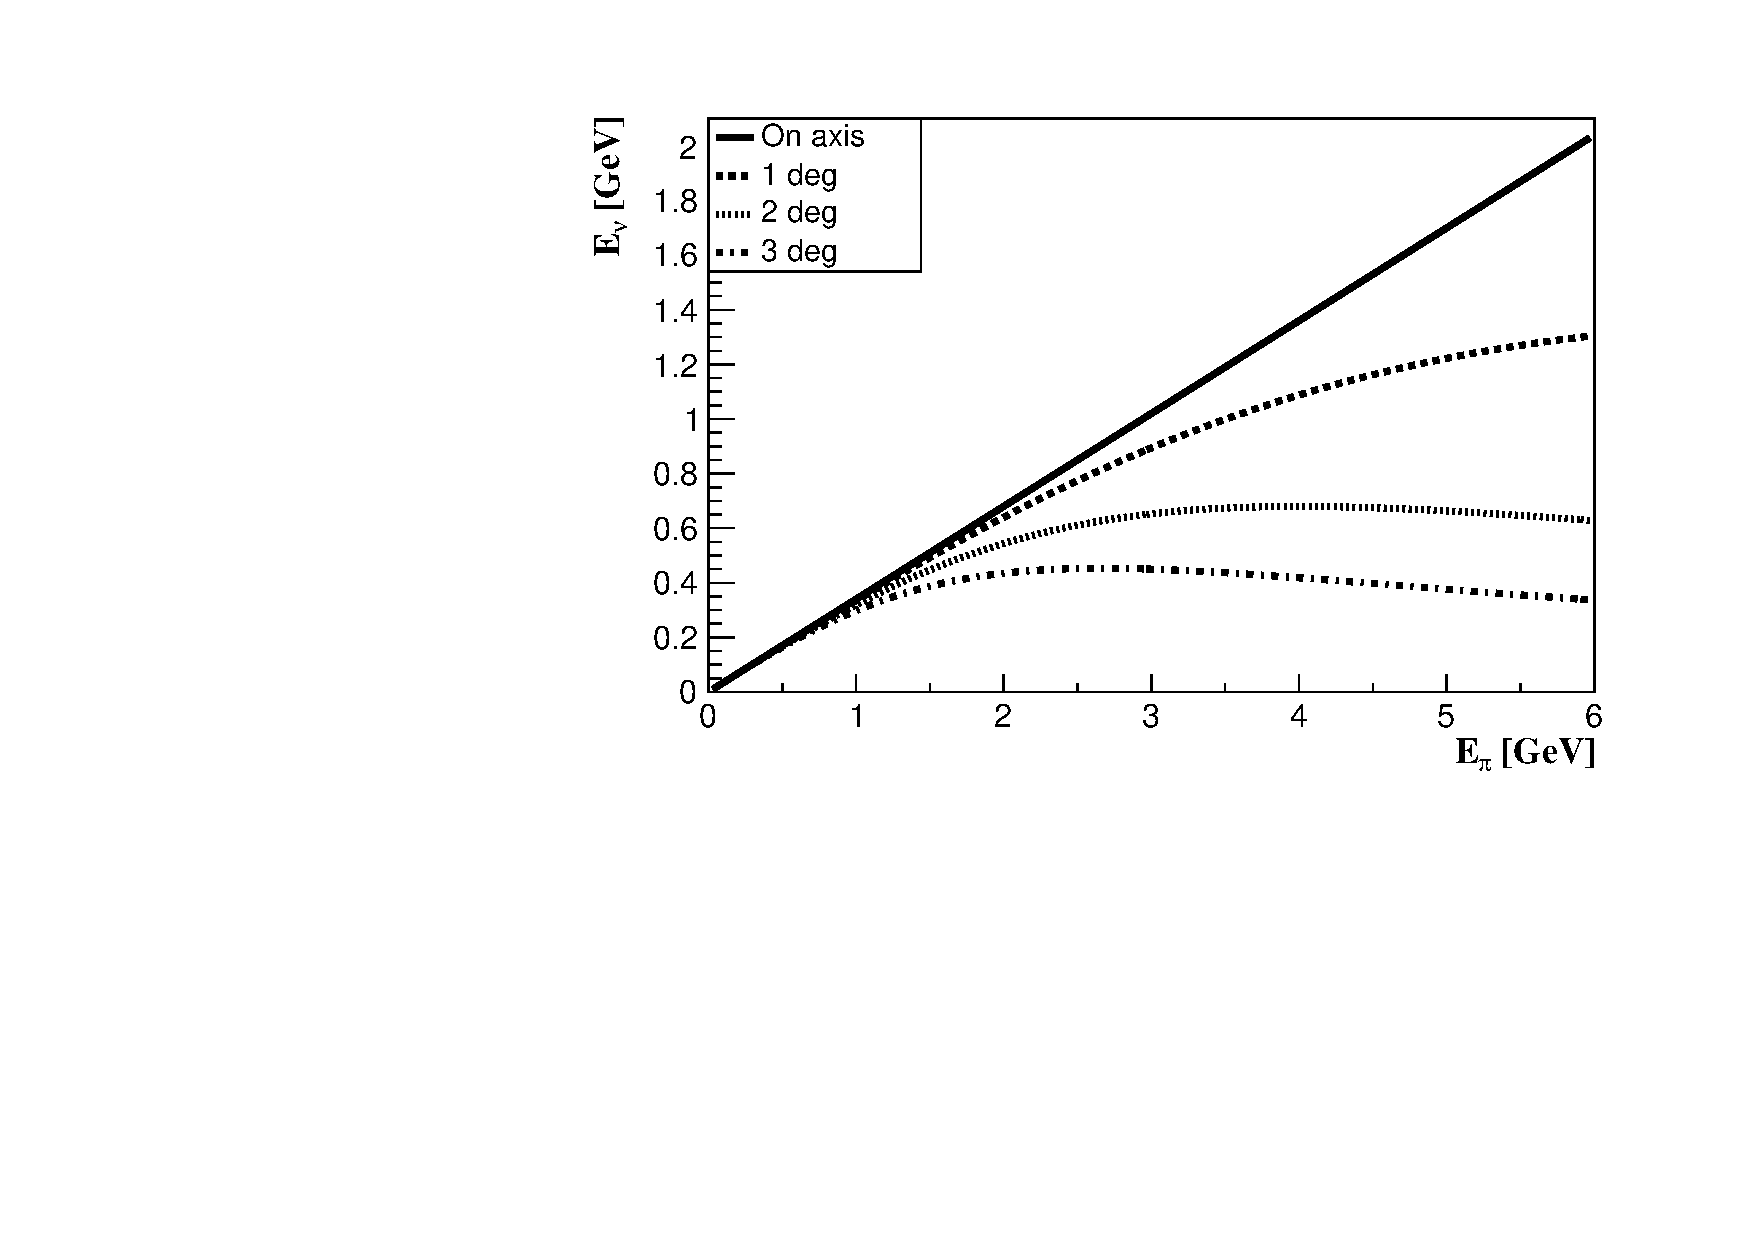
\includegraphics[width=0.6\linewidth]{figures/offaxis.pdf}
  \caption{Neutrino energy as a function of the pion energy for on-axis decays and several off-axis angles. For a non-zero off-axis angle, the neutrino energy reaches a maximum. This feature is currently exploited in the T2K and \nova experiments.}
 \label{fig:offaxis}
 \end{figure}


As the neutrino beam is a tertiary beam, it is necessary to include in the experimental apparatus monitoring devices to ensure that it is stable in intensity and direction. To this effect, muon detectors, sensitive to the muons produced by the pion decays, are placed close to the end of the decay volume. Moreover, as the neutrino flux and cross-sections and the beam composition are not known with sufficient precision, a near detector is located close to the target station (typically within a few hundred meters). The near detector constrains the neutrino interaction rate, proportional to the product of the neutrino flux and the cross-section. Moreover, the near detector allows to measure the beam composition and to perform the study of several neutrino cross-sections.    

For recent long-baseline experiments, it is especially important that the beam is very pure in $\nu_\mu$. An irreducible $\nu_e$ component, at the percent level, is always present, due to the K$_{e3}$ semileptonic decays of kaons and to the decays of muons, produced by the pions.

In the antineutrino mode, the fraction of neutrino interactions is relatively large. For instance, in the case of T2K, roughly 30\% of the interactions at SK in antineutrino mode are produced by neutrinos. This is due to the the fact that more $\pi^+$ than $\pi^-$ are produced in proton-carbon interactions and that \nunu cross-section are larger than \nub cross-sections. 
These impurities in the beam need to be measured, for instance with a magnetized near detector. 

\begin{table}
\centering
\caption{Parameters of recent and future long-baseline experiments. Energy and power refer to the primary proton beam, L is the baseline, FD the mass of the far detector. POT (Protons On Target) represents the integrated dataset as of 2016 for the running experiments, and the total foreseen exposure for future projects.}
\begin{tabular}{|c|c|c|c|c|c|}
  \hline
  Exp. & Energy (GeV) & Power (kW) & L (km) & FD mass (kt) & POT \\ 
  \hline
K2K & 30 & 27 & 250 & 50 & 9.2 $\times$ 10$^{19}$\\
MINOS & 120 & 700 & 790 & 5.4 & 8.2 $\times$10$^{20}$\\
OPERA & 450 & 300 & 730 & 1.8 & 1.8 $\times$10$^{20}$\\
T2K & 30 & 750 & 295 & 50 & 2 $\times$10$^{21}$\\
\nova & 120 & 700& 810 & 14 & 6 $\times$ 10$^{20}$\\
HK & 30 & 1300 & 295 & 380 & 2.7 $\times$ 10$^{22}$\\
DUNE & 80 & 1070 & 1300 & 40 & 1.3 $\times$ 10$^{22}$\\
  \hline
\end{tabular}
\end{table}

\subsection{Detectors for long-baseline experiments}

The neutrino detectors in long-baseline experiments are quite similar to those used for atmospheric neutrinos, as the energy range of interest is similar. Moreover, in both cases, a very massive (tens of kt or more) underground detector is needed and therefore the same detector can be used to study both sources. An example is Super-Kamiokande (see subsection~\ref{subsec:atmevidence}) which is also used as the far detector for the long baseline T2K experiment. 
Besides the detection of muons produced by $\nu_\mu$ interactions to probe the disappearance channel, the emphasis has been shifting recently to the study of $\nu_e$ appearance. This requires to discriminate between electron showers produced by CC reactions like for instance $ \nu_e n \rightarrow e p$ and NC reactions like $\nu n \rightarrow \nu \pi^0 + X$.
Four main far detector technologies have been used or considered: 
\begin{itemize}
\item The water Cherenkov detection technique. It is used by Super-Kamiokande and has several advantages as it is well demonstrated and allows to instrument large detector masses. It is specially effective in the sub-GeV energy range where CCQE processes dominate the cross-section producing single Cherenkov ring which are easier to reconstruct and measure. For fully contained events, the total lepton energy can be reconstructed and the neutrino energy inferred from the CCQE kinematics. This technique is the only candidate to instrument very large detector masses approaching the megaton scale.
A similar technique is used by the IceCube and ANTARES experiments in an open natural medium, the Antarctic ice and deep under sea.
\item The magnetized iron-scintillator calorimeters like MINOS. They offer the advantage of measuring the charge of penetrating tracks, however they are limited by their ability to distinguish $\nu_e$ from NC $\pi^0$ production.
\item Totally active scintillator detectors like NOvA. Here the detection medium is a liquid scintillator contained in plastic cells read out by optical fibers.
\item Liquid Argon Time Projection Chambers. This is a new technology pionereed by the ICARUS experiment, that has been chosen for the future DUNE experiment. This detector offers superior performances in terms of information on the particles produced in the final state, with the possibility of particle identification and total energy reconstruction. A large program of R\&D is on-going at Fermilab and CERN to demonstrate the feasibility of this technology for large detectors of 10 kt.
\end{itemize}

 

\subsection{Flux and cross-section systematic uncertainties}
\label{sec:beamsyst}

Long-baseline neutrino oscillation experiments require a good control of the systematic uncertainties related to neutrino fluxes and neutrino cross-sections to perform precision measurements of oscillation parameters. 

A common strategy to reduce systematic uncertainties, used in most of the long baseline experiments, is the use of a Near Detector complex, located few hundreds of meters from the beam target. In this way the neutrino spectrum and the flavour composition of the beam can be precisely measured before the oscillations and this is used to determine the expected spectra at the far detector.

Some long-baseline experiments, for example MINOS and \nova, use near detector  that have the same composition and technology as the far detector, so that cross-section uncertainties due to the different target nuclei or detector systematic uncertainties are minimized in the extrapolation. Other experiments, for example K2K and T2K, use a set of near detectors with different target nuclei in order to maximize the information on the cross-section models.

In this section, as an example, we will briefly describe how the T2K experiment uses the near detector data to reduce the systematic uncertainties in the oscillation analysis~\cite{t2kprd}. The T2K near detector, called ND280, is magnetized, with several sub-detectors installed within the ex-UA1/NOMAD magnet that provides a 0.2 T magnetic field. For the oscillation analysis, the ND280 tracker system is used, comprising two Fine Grained Detectors (FGD) interleaved with three Time Projection Chambers (TPCs). The FGDs act as an active target for neutrino interactions (each with a mass of about 1~ton). Particles produced in the FGD enter the TPCs where the charge and the momentum of the tracks is reconstructed and the particle identified based on the measurement of the energy loss in the gas. One important point to notice is that one of the two FGDs is a fully active detector, while in the second one scintillator layers are interleaved with inactive water layers, allowing to select neutrino interactions on carbon and on oxygen, the same target as the far detector, SK. 
    
At T2K energies, most of the \num charged current neutrino interactions are quasi-elastic events, producing only one visible track in the final state, the muon since the proton has often a low momentum around 200 MeV/c and its track is too short to be reconstructed. The presence of the magnetic field allows to reconstruct the charge of the muons, distinguishing between negative muons produced by \num and positive muons produced by \numb interactions.
In some cases neutrinos exchange enough energy with the target nuclei producing also pions or protons that can, in some cases, enter the TPC. 
For \num selections, ND280 distinguishes three cases on the basis of the final state topology: only the muon is reconstructed (CC0$\pi$, with a 63 \% purity of CCQE events), the muon and one negative pion is also reconstructed (CC1$\pi$) and events with more pions (CCother, essentially deep-inelastic events). For \numb selections interaction with one track are separated from the interactions with more than one track. The total sample selected in ND280 comprises about 25000 events.
  
The same selections are applied to interactions in both the FGD and all the samples are then fit to reduce systematic uncertainties on the flux and cross-section model. 
The main uncertainty on the flux model is due to the hadron production cross-section. Data from the NA61/SHINE experiment at CERN are used. In NA61/SHINE a proton beam is accelerated to 30 GeV/c and strikes a target. Hadrons produced are measured with a system of TPCs and Time Of Flight detectors, and double differential cross-section (in angle and momentum) are extracted. Thanks to NA61/SHINE data the uncertainties on the neutrino fluxes, prior to the ND280 fits, are reduced to the 10-15\% level.

For the cross-section model, the priors are based, as much as possible, on external experiments such as MiniBooNE and MINERvA. An important aspect is that, for the first time, effects related to the multi-nucleon 2p-2h emissions are included in this analysis, based on the Nieves et al. model~\cite{Nieves:2011yp}

To reduce flux and cross-section uncertainties, the ND280 samples are binned in the kinematic variables \ptheta according to the muon momentum and angle with respect to the beam direction. Data and Monte Carlo are fitted using a binned likelihood, where the prediction for each bin depends on the flux, cross-section and detector systematic parameters. 

The result of the fit is a set of point estimates and covariance for the systematic scaling factors for the unoscillated neutrino flux at SK. The impact of the ND280 fit on the total error budget in the T2K oscillation analysis is shown in Table~\ref{tab:t2ksyst}: a reduction of the systematic uncertainties from $12\%$ to $\sim5\%$ is obtained thanks to the near detector fit.

\begin{table}[htb]
\begin{center}
\caption{Sources of the systematic uncertainty on the predicted neutrino event rates at Super-Kamiokande in T2K oscillation analyses.
The effect of the near detector constraint (ND280) on the flux and cross-section is particularly visible. The line (Other) reports the effect of Final State Interactions and Secondary Interactions.
}
\begin{tabular}{|l|c|c| } \hline 
Source of Uncertainty& $\nu_e$ & $\nu_{\mu}$ \\ 
 &$\delta N/N$&$\delta N/N$\\ \hline
Flux&3.7\%& 3.6\% \\ \hline
cross-section &5.1\%& 4.0\% \\ \hline
Flux+cross-section&& \\
(w/o ND280 Constraint)&11.3\% &10.8\% \\
(w/ ND280 Constraint)&4.2\% &2.9\% \\ \hline
Other & 3.5\%& 4.2\% \\ \hline
All & & \\
(w/o ND280 Constraint)& 12.7\%& 12.0\% \\ 
(w/ ND280 Constraint)& 6.8\%& 5.1\% \\ \hline 
\end{tabular}
\label{tab:t2ksyst}
\end{center}
\end{table}


In the case of \nova, they profit of the fact that the near and the far detector are identical and use a calorimetric approach in which all the energy observed in the event at the near detector is reconstructed and is then unfolded to obtain the expected true neutrino energy. The far to near ratio and the oscillation probabilities are then applied to obtain the expected true energy spectrum at the far detector. This method allows to reduce the total systematic uncertainty to level similar to the ones obtained by T2K.

\subsection{Results from long-baseline accelerator experiments}

K2K (KEK-to-Kamioka) was the first long baseline neutrino beam, using Super-Kamiokande as its far detector at 250 km from the neutrino production source. Operating between 1999 and 2004, it has measured the disappearance of $\nu_\mu$ governed by Eq.~(\ref{eq:mudisapp}): 112 events were observed, while 158.1$^{+9.2}_{-8.6}$ were expected without oscillation, a 4.3 $\sigma$ effect~\cite{Ahn:2006zza}. This measurement has confirmed neutrino oscillation as the explanation for the atmospheric neutrino disappearance. 

Further improved measurements of the $\nu_\mu \rightarrow \nu_\mu$ oscillations were reported by MINOS, a long baseline experiments with a neutrino beam from Fermilab to the Soudan mine in Minnesota (baseline 735 km). Protons from the Main Injector with an energy of 120 GeV were used with a tunable setup, allowing to vary the neutrino energy and mostly used in the position giving a 1-3 GeV neutrino beam.
The far detector was a 5.4 kton magnetized steel-scintillator calorimeter. In 2011, MINOS~\cite{minos11} reported a measurement of $|\Delta m^2_{31}| = 2.32 {}^{+0.12}_{-0.08} \times 10^{-3}$ eV$^2$ and $\sin 2 \theta_{23} > 0.90$ at 90\% C.L.   

The current generation of experiments, T2K and \nova, use a narrow band beam, based on the off-axis design, that is particularly suited for the measurement of \num disappearance once the relevant squared mass difference is known. For a given \dmsq and a given baseline distance, in fact, the oscillation probability depends on the neutrino energy that can be tuned by changing the off-axis angle. In the case of T2K (L=295~km) the maximum of the oscillation is at an energy of 600 \mev while in the case of \nova  (L=810~km) the maximum is at 1800 \mev. 

While the most recent analyses published by T2K do a global fit of appearance and disappearance modes to extract the maximum of the information on neutrino oscillations in the PMNS framework, disappearance analyses only have also been done by T2K in order to test the PMNS framework. In the \num disappearance probability in fact there are no CP odd terms so the disappearance probability is expected to be the same for \num and \numb. Previous results from MINOS showed some tensions between neutrinos and antineutrinos. Differences between neutrinos and antineutrinos oscillation probabilities in this channel can be due to CPT violation.

For the T2K experiments, fully contained \num events are selected in Super-Kamiokande in time with the beam, with one ring identified as produced by a muon and less than two decay electrons. The resulting sample is composed by 62 \% of CCQE $\nu_\mu$ events, 32 \% of non-CCQE $\nu_\mu$ events and the rest essentially by NC events.
Based on \nupot protons-on-target (POT) collected in neutrino mode and \nubpot POT collected in antineutrino mode, T2K has observed 135 (66) \num (\numb) candidates at SK with 522 (185) events expected in case of no-oscillations and 135.8 (64.2) events expected for maximum disappearance. The reconstructed energy spectrum for both, \num and \numb surviving events are shown in Fig.~\ref{fig:t2kdis}. Thanks to the use of the Near Detector data described in Sect.~\ref{sec:beamsyst}, the systematic uncertainties on these measurements are at the 5\% level and a precise measurement of \thatm and \dmsq is obtained as shown in Fig.~\ref{fig:atm-nunubar}. The oscillation parameters measured are in excellent agreement between neutrinos and antineutrinos and both are compatible with maximal mixing for \thatm.

\begin{figure}[htbp]
\centering
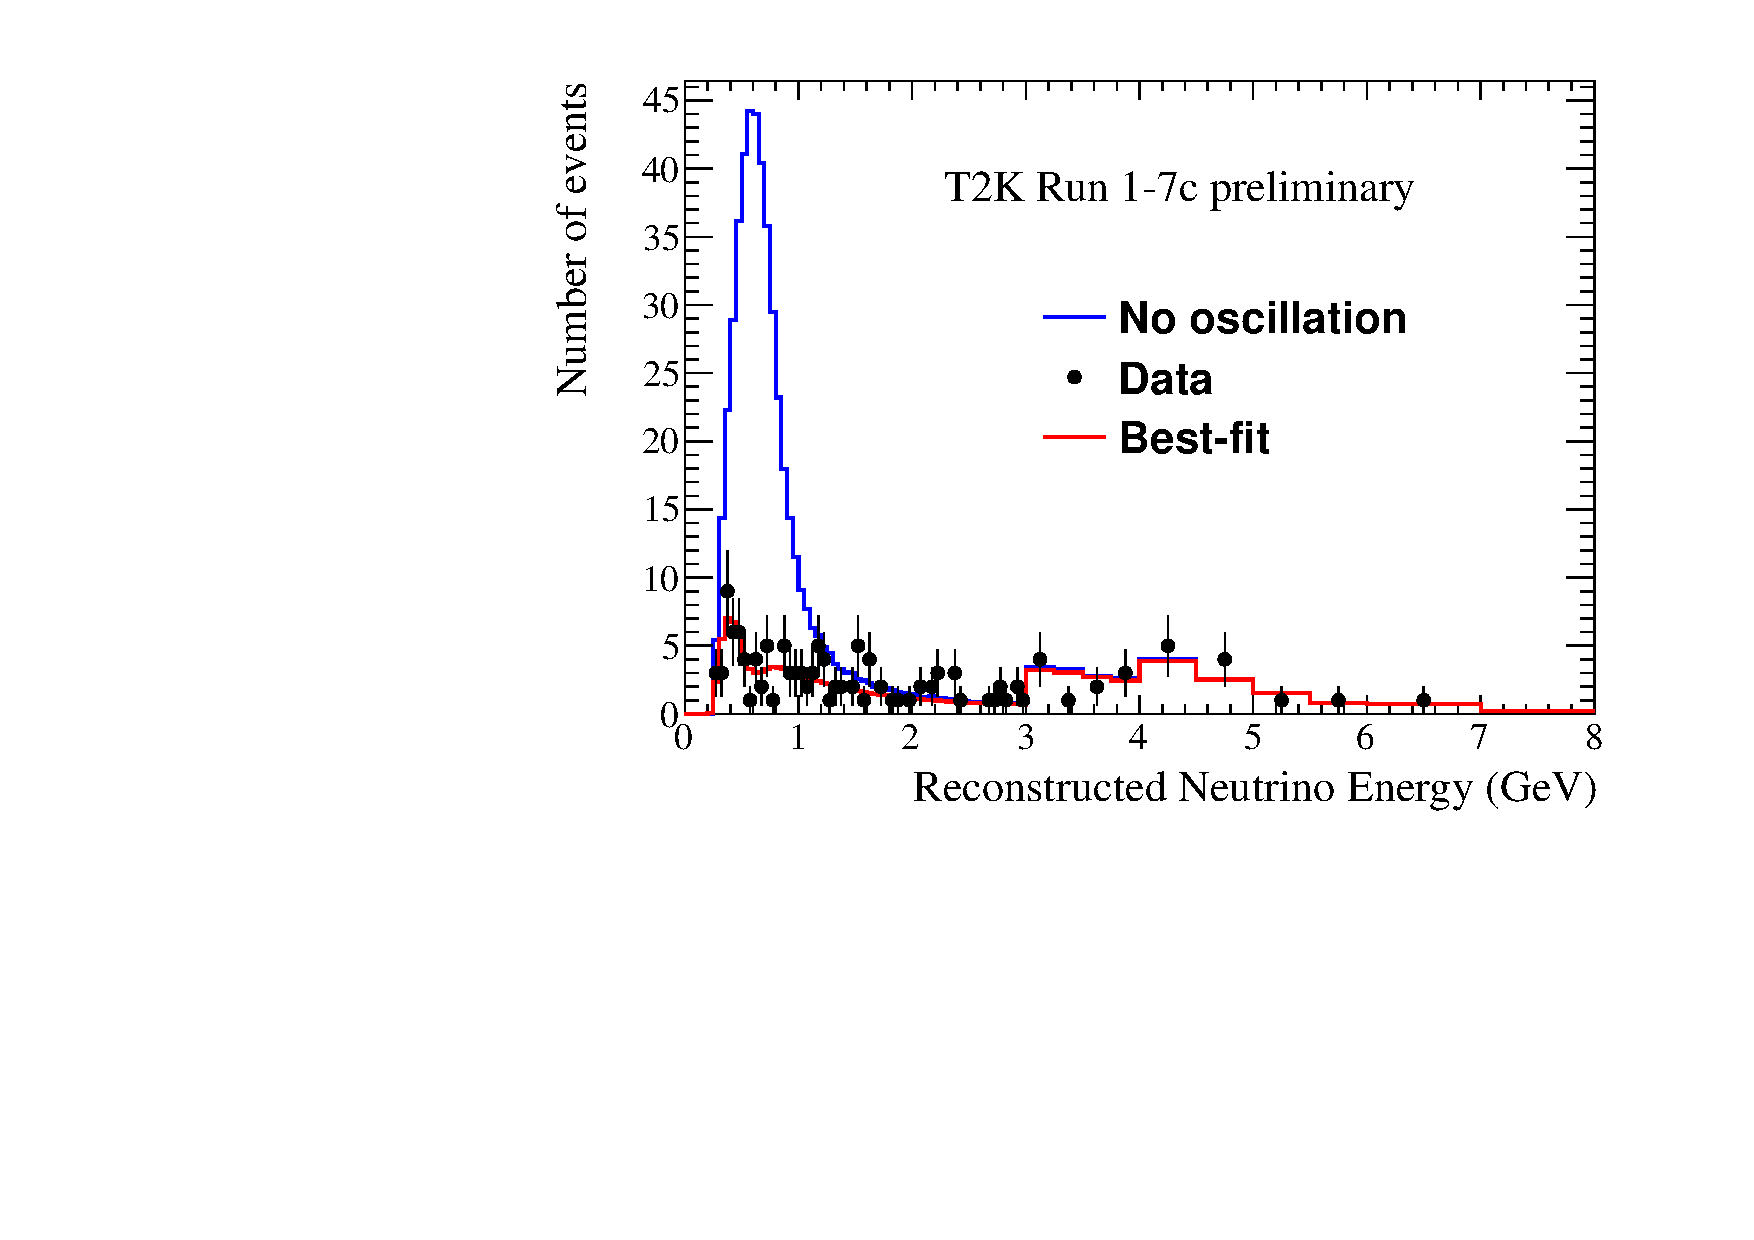
\includegraphics[width=0.4\linewidth]{figures/bestfit_sinsqth23vsdcpvsmh_1rmu_run17.pdf}
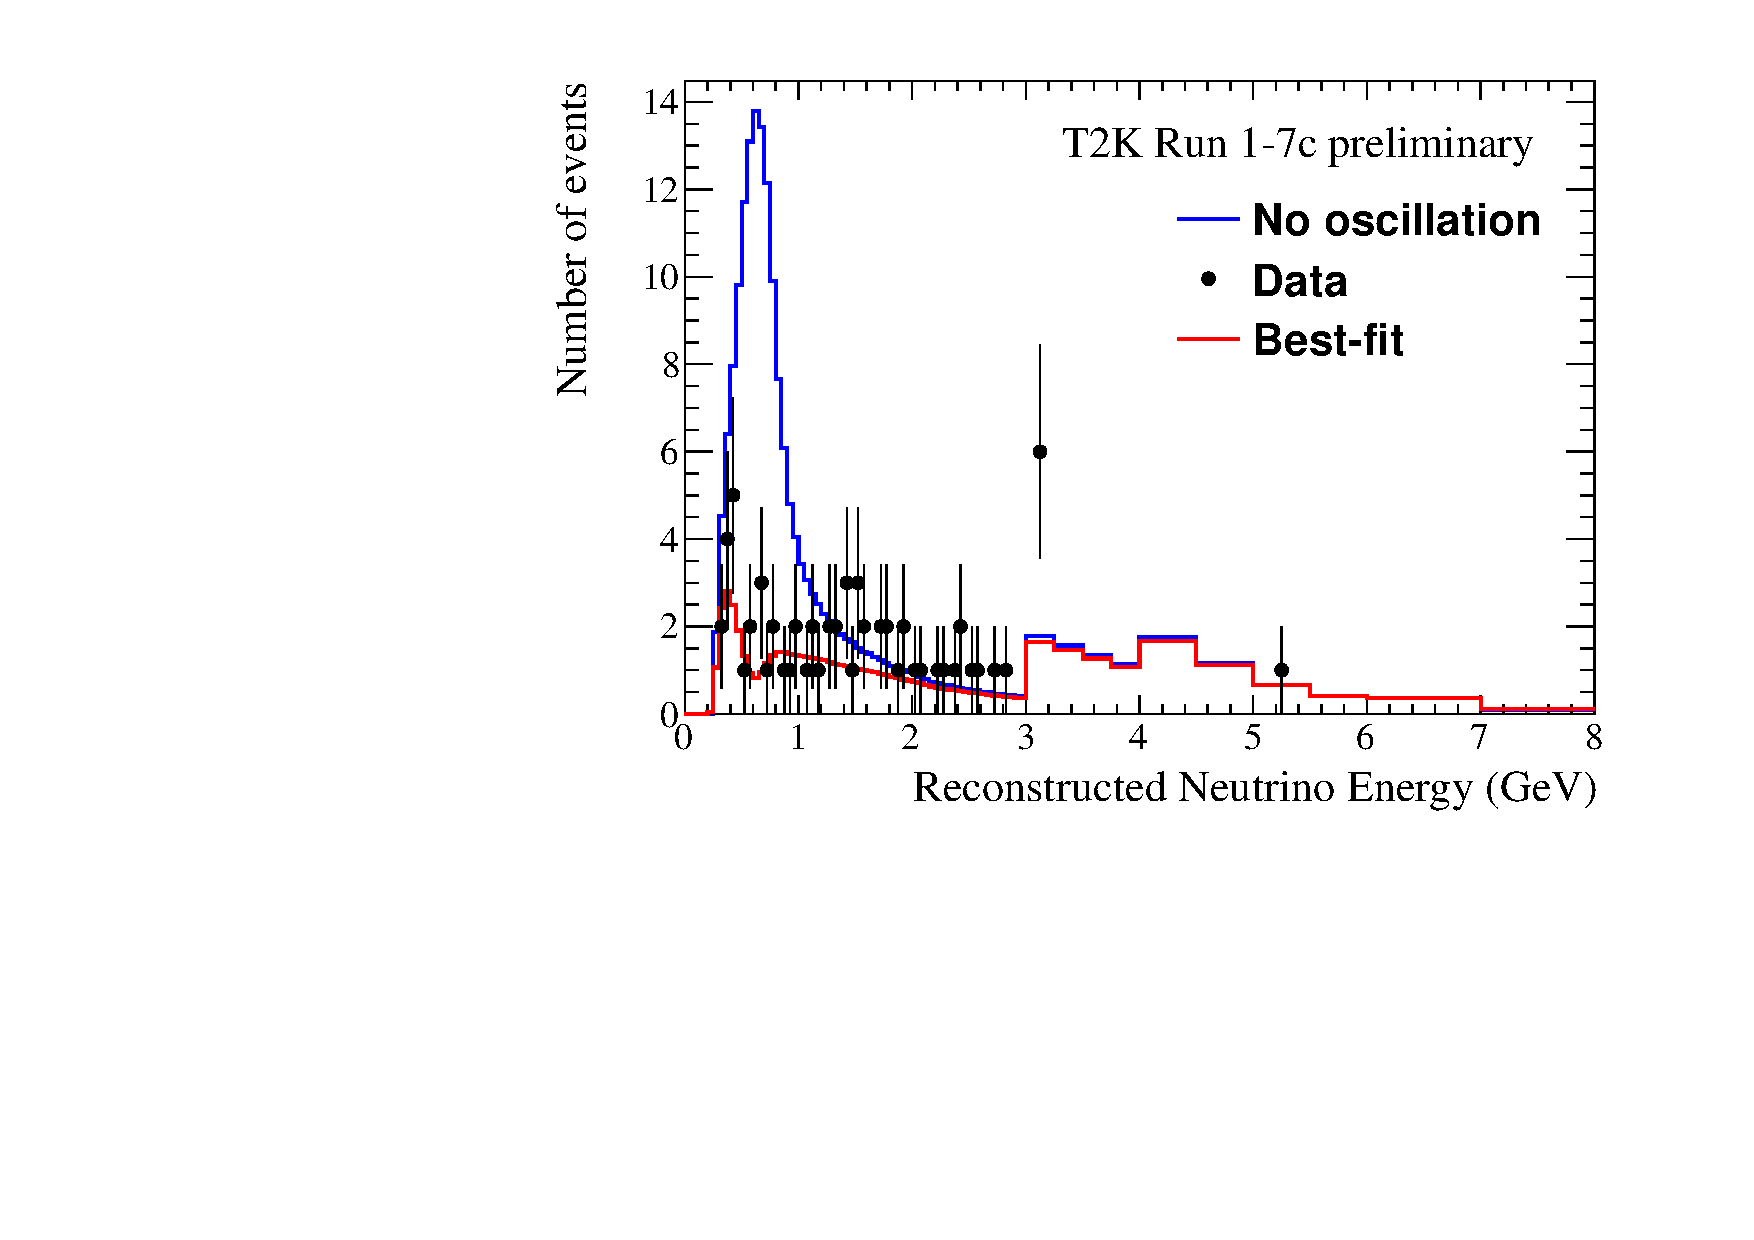
\includegraphics[width=0.4\linewidth]{figures/bestfit_sinsqth23vsdcpvsmh_rhc1rmu_run17.pdf}
  \caption{
Reconstructed \num and \numb energy spectrum at the far detector by the T2K collaboration for data, best-fit prediction, and
unoscillated prediction. Courtesy of the T2K collaboration. %Bottom: Ratio of oscillated to unoscillated events as a function of
%neutrino energy for the data and the best-fit spectrum.
}
 \label{fig:t2kdis}
 \end{figure}

\begin{figure}[htbp]
\centering
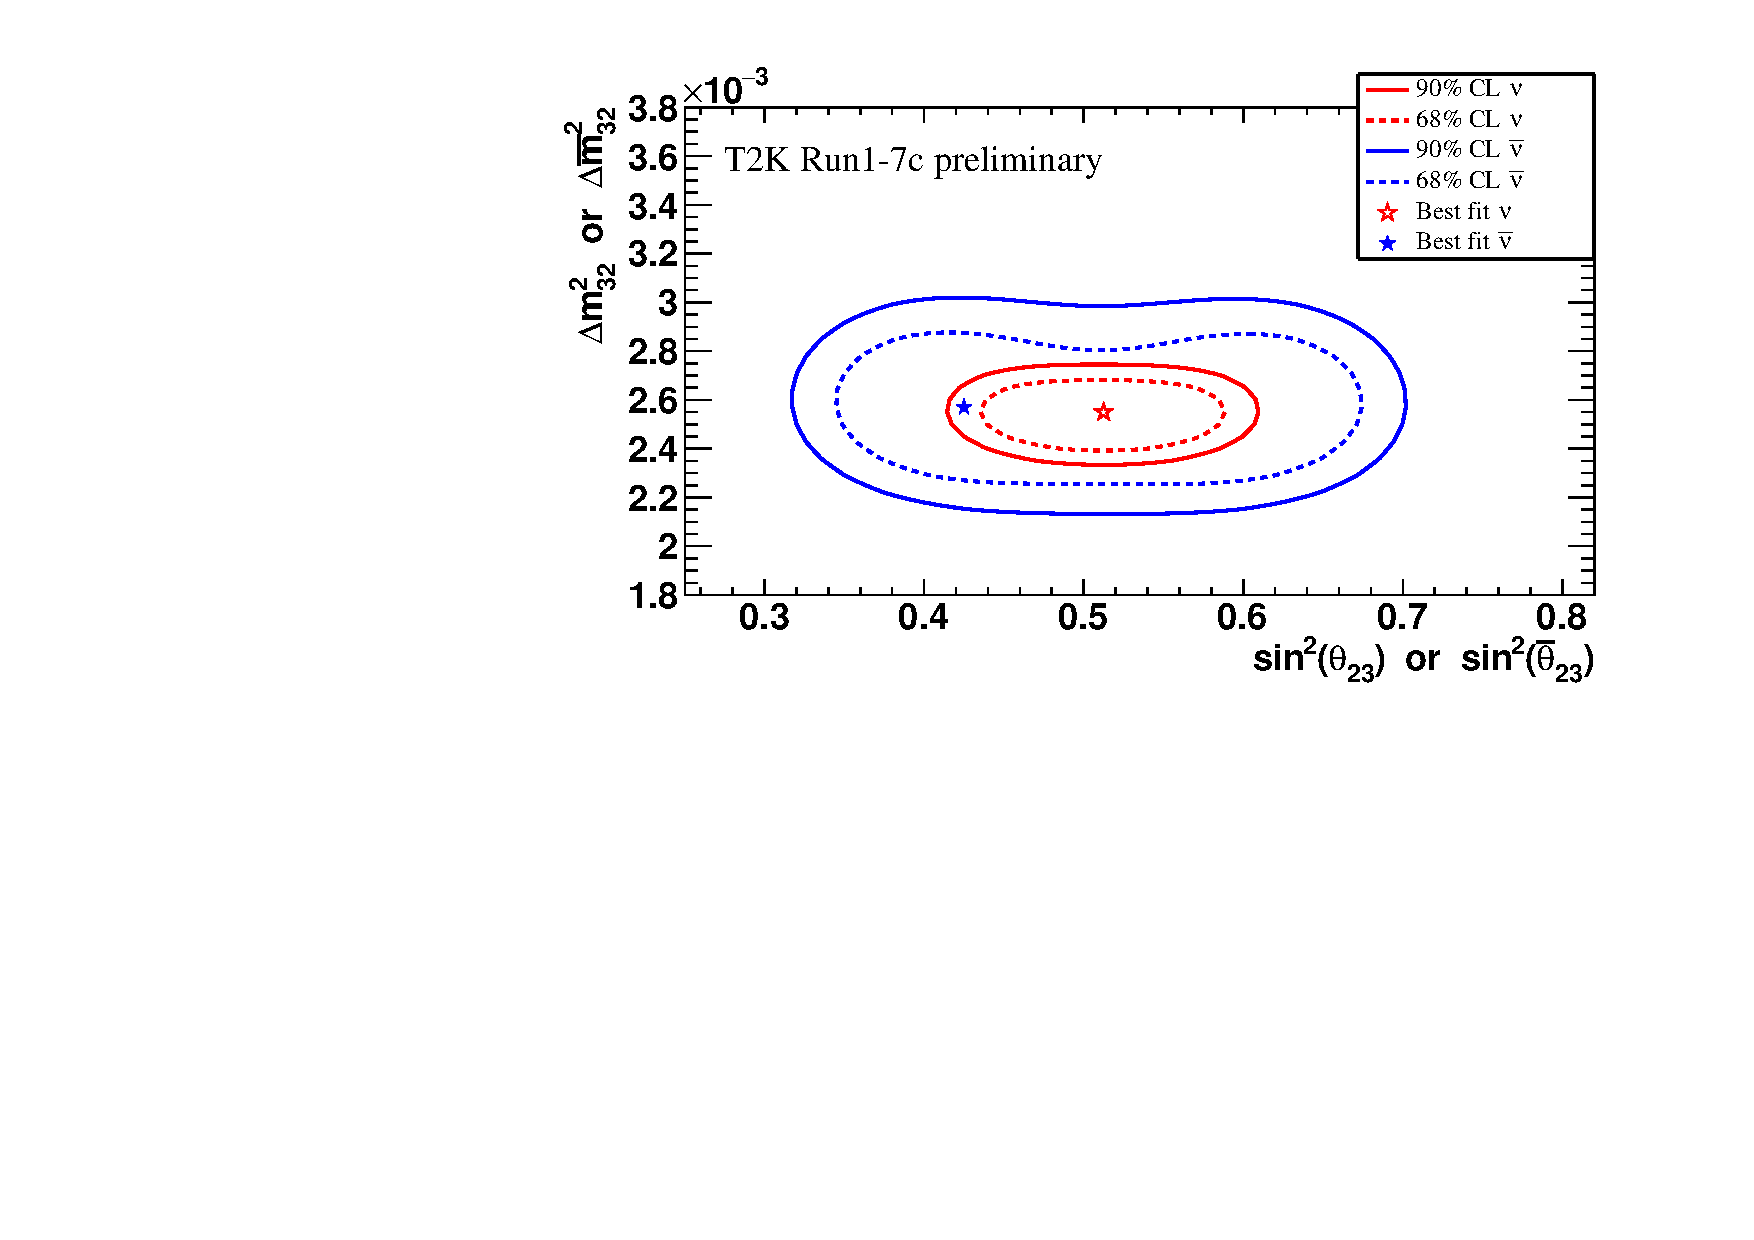
\includegraphics[width=0.6\linewidth]{figures/nu_vs_nubar_datafit_17c_nh.pdf}
  \caption{T2K measurement of $\Delta m_{32}^2 $ versus \stt for neutrinos and antineutrinos. The solid (dashed) contours show the 90\% (68\%) C.L. regions, while the stars show the best-fit points. Courtesy of the T2K collaboration.}
 \label{fig:atm-nunubar}
 \end{figure}

\nova has also reported a measurement of \num disappearance using \novapot POT and selecting \mmu-like candidates at the far detector~\cite{Adamson:2017qqn}. They observed 78 events in the far detector, while $473\pm30$ were expected without oscillations. This result leads to some tensions, especially with the T2K experiment, since maximal mixing is excluded by \nova at $2.5\sigma$ as shown in Fig.~\ref{fig:atm-contour}. 

\begin{figure}[htbp]
\centering
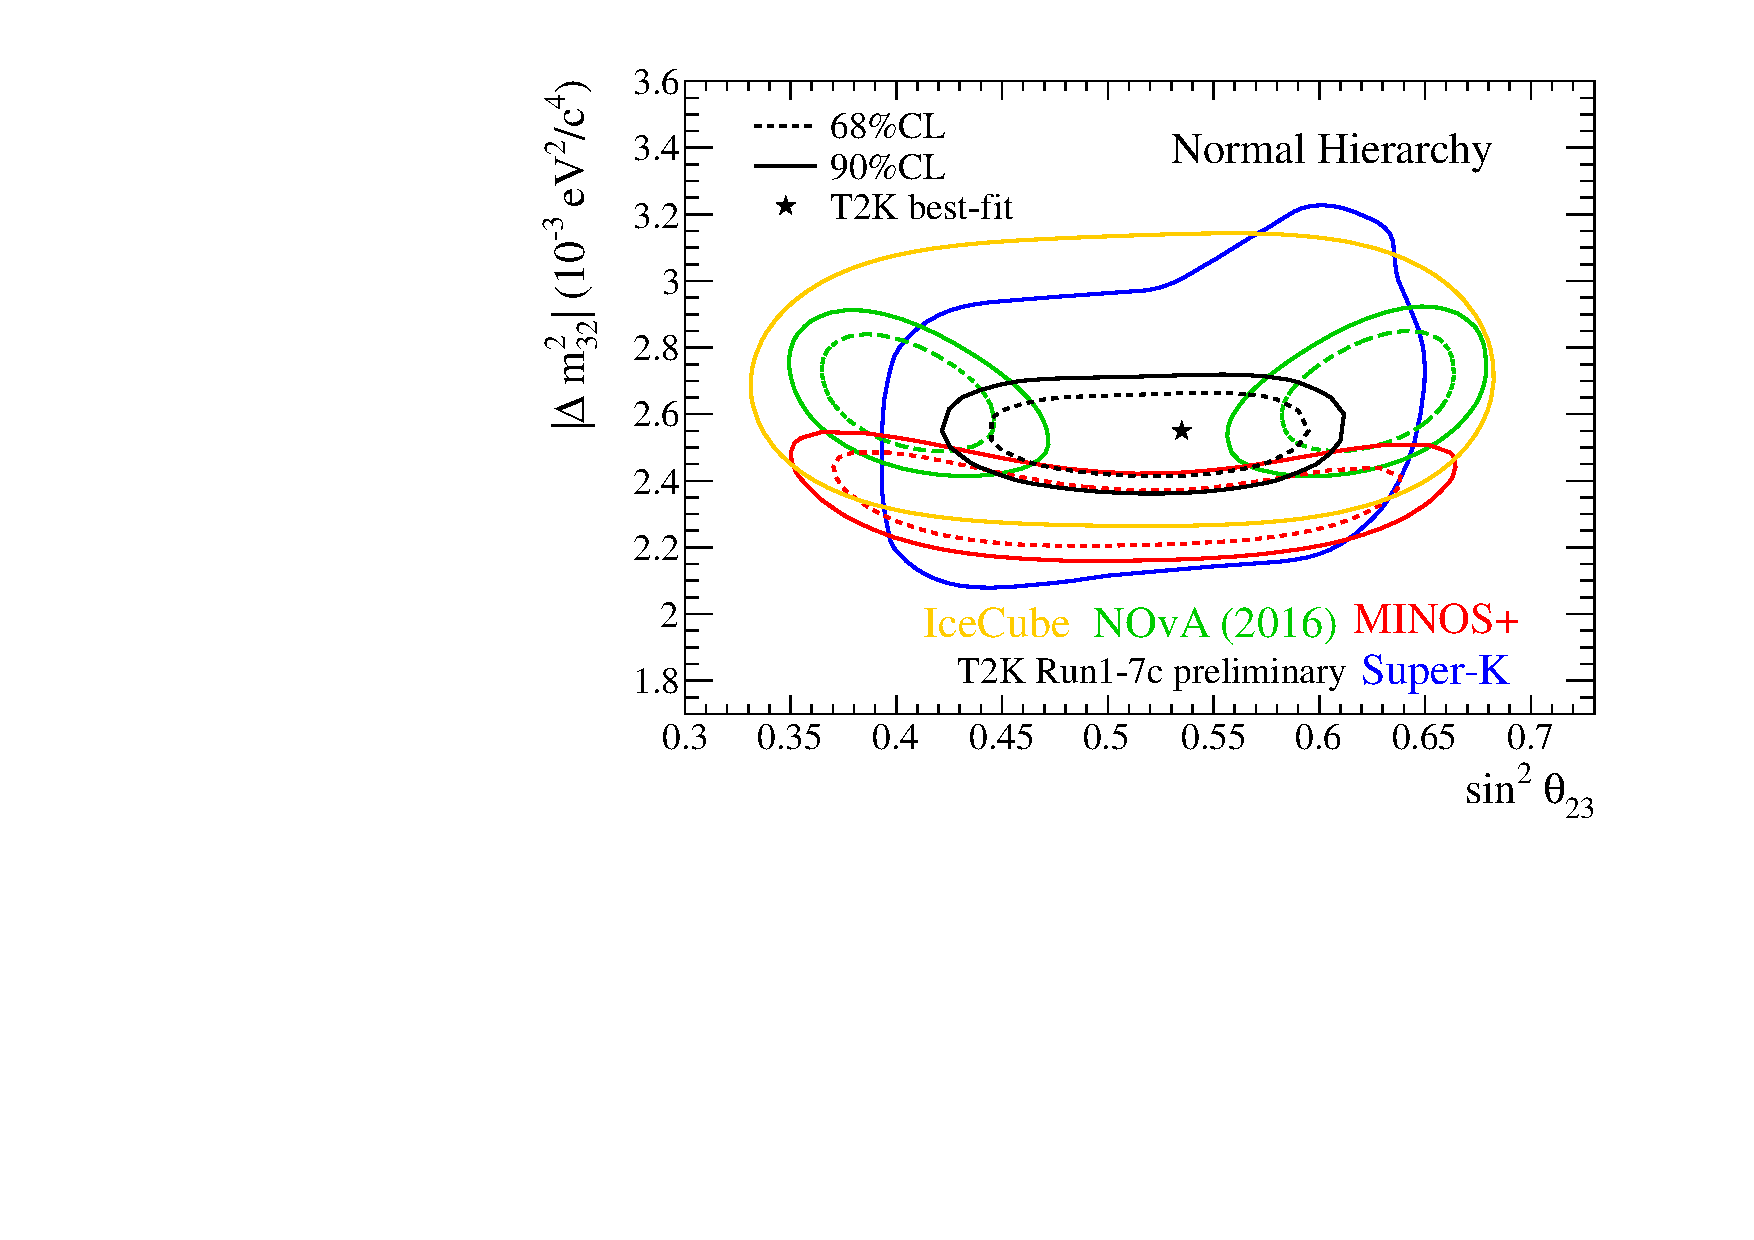
\includegraphics[width=0.5\linewidth]{figures/sinsqth23vsdmsq_react_othexp_nh.pdf}
%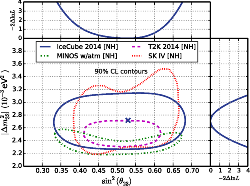
\includegraphics[width=0.6\linewidth]{figures/atm-contour.pdf}
  \caption{
Confidence regions in the plane   $\Delta m^2_{32} (\Delta m^2_{13})$ versus $\sin^2 \theta_{23}$, for T2K~\cite{t2k2016}, Super-K~\cite{Wendell:2015onk}, Minos+~\cite{PhysRevLett.110.251801}, \nova~\cite{Adamson:2017qqn} and IceCube DeepCore~\cite{Aartsen:2016psd}. Courtesy of the T2K collaboration.}
 \label{fig:atm-contour}
 \end{figure}
 
The two collaborations are working to understand this difference that could still be simply due to statistical fluctuations. A comparison between the reconstructed energy spectrum for the best-fit and the one obtained by imposing maximal mixing in \nova is shown in Fig.~\ref{fig:atm-nova}. Similarly T2K data are compared with the T2K best fit and the spectrum obtained by imposing the NOvA best-fit oscillation parameters as shown in Fig.~\ref{fig:t2kdiscomparison}. Additional data from T2K and NOvA will help clarify the situation. 
 
 \begin{figure}[htbp]
\centering
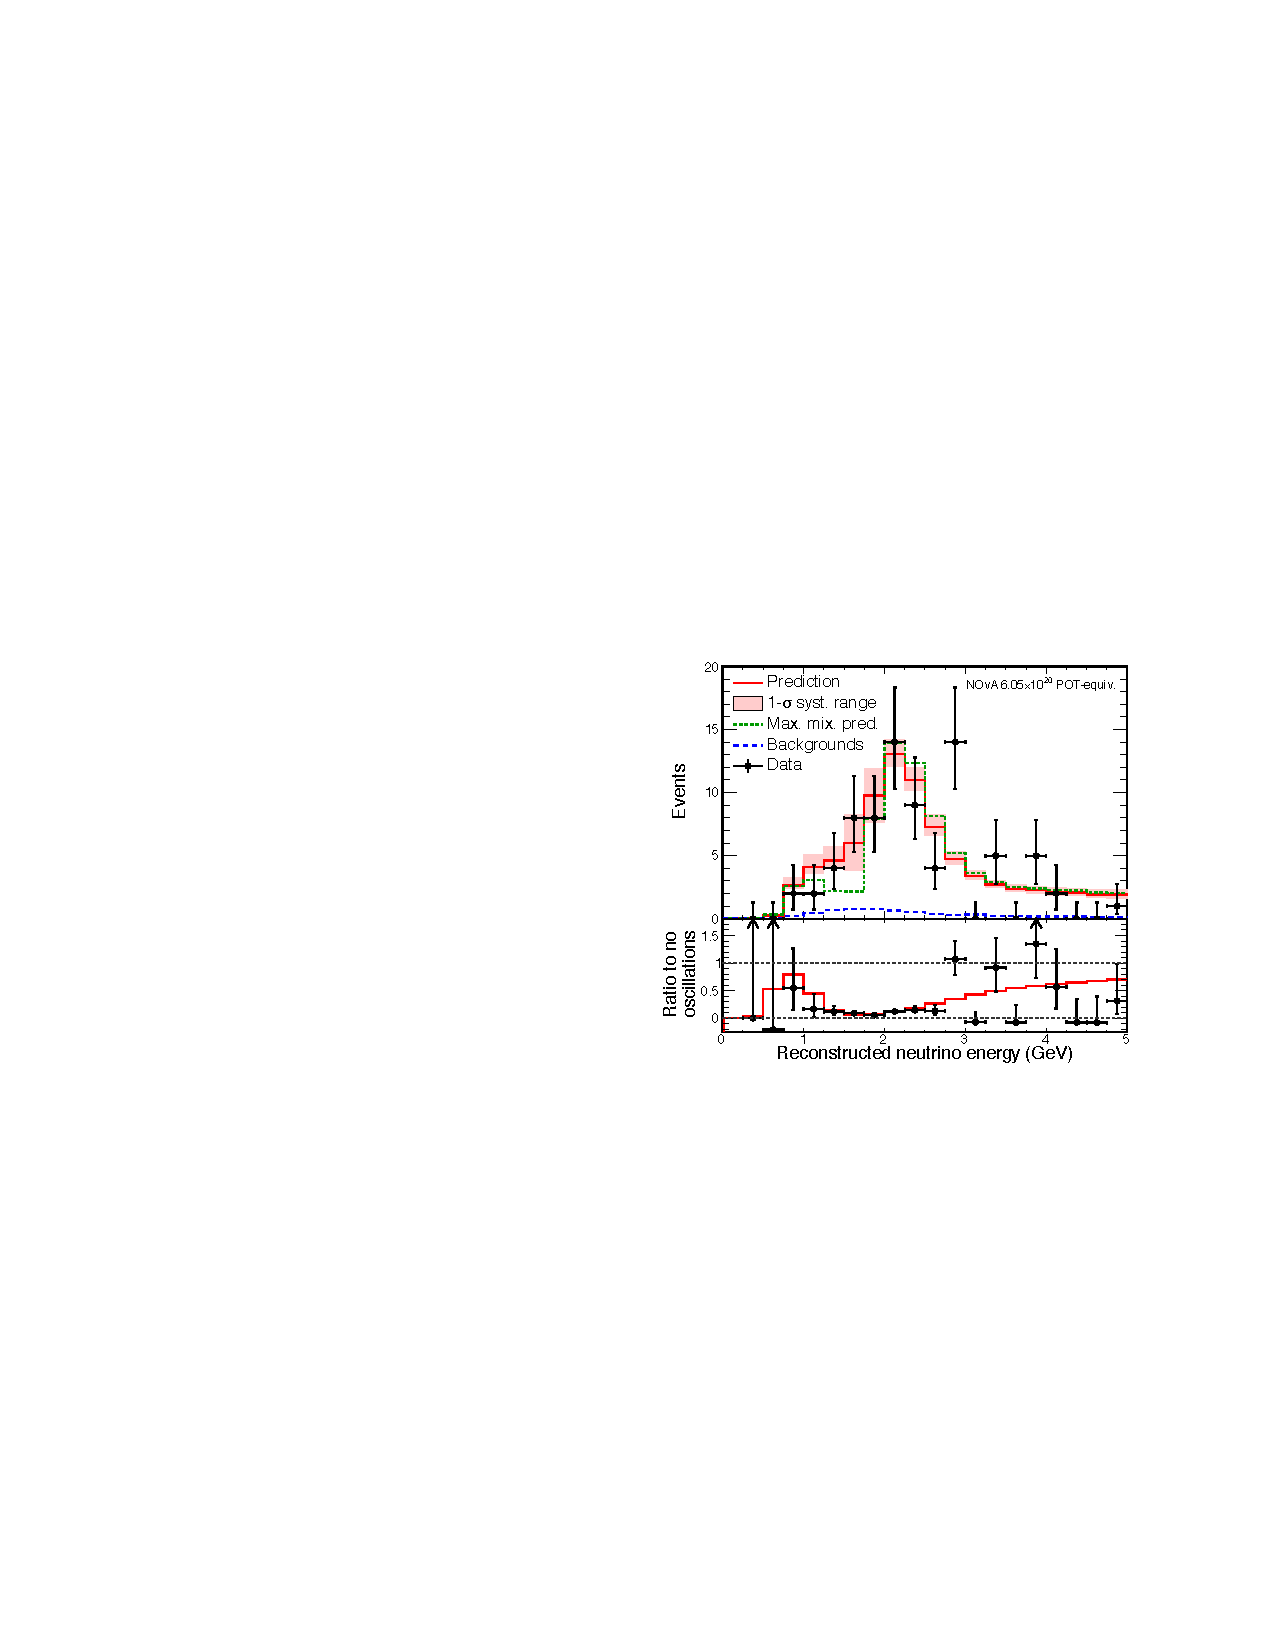
\includegraphics[width=0.6\linewidth]{figures/nova_numudisappearance.pdf}
  \caption{Reconstructed energy spectrum for \num candidates in \nova for the data (black dots), the best fit (solid red line) and the prediction assuming maximum mixing angle $\theta_{23}$ (dashed line)~\cite{Adamson:2017qqn} Courtesy of the \nova collaboration.}  \label{fig:atm-nova}
 \end{figure}
  
 \begin{figure}[htbp]
\centering
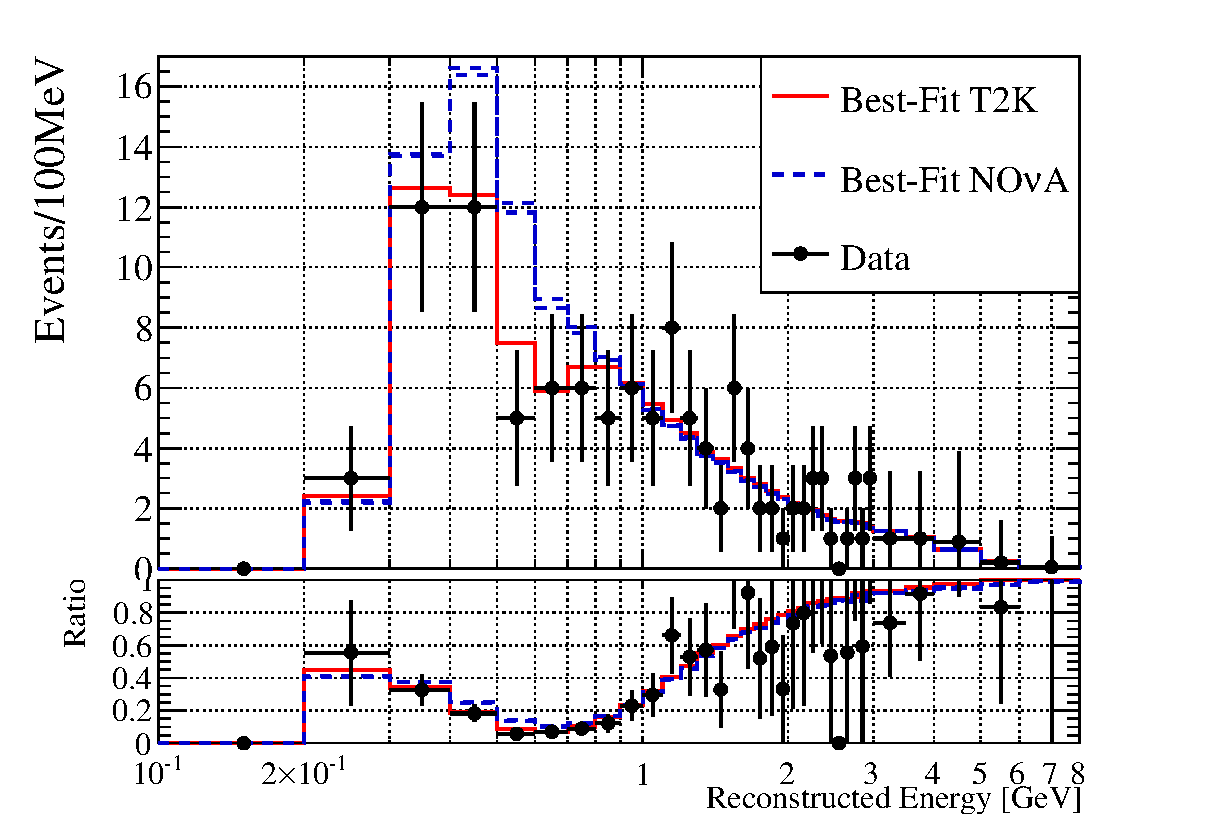
\includegraphics[width=0.6\linewidth]{figures/MC_marg_data_Run1-7c_RC_numu_log_ratio_density_nova.eps}
  \caption{Reconstructed energy spectrum for \num candidates in T2K for data (black points), T2K best fit (red solid line) and the prediction assuming \nova best fit values (dashed line). Courtesy of the T2K collaboration.} \label{fig:t2kdiscomparison}
 \end{figure}
 
 \subsection{Evidence for $\nu_\tau$ appearance}

The OPERA experiment on the CERN to Gran Sasso neutrino beam, taking data between 2008 and 2012, was designed to test the $\nu_\mu \rightarrow \nu_\tau$ appearance hypothesis. The detector is based on the Emulsion Cloud Chamber technique, with 1800 ton of nuclear emulsion detectors in the forms of bricks, each brick being composed of a stack of nuclear emulsion films and lead plates. This target, capable of sub-micrometric track resolution, is devoted to the study of the neutrino interaction vertex and the particles associated to it. The identification of the $\tau$ leptons relies mainly on their characteristic kink (Fig.~\ref{fig:opera}) due to the decay $\tau \rightarrow h \nu_\tau$, or $\tau \rightarrow l \nu_\tau \bar \nu_l$, where $h$ is a charged meson, and $l$ is an electron or a muon. Another signature is related to the decay $\tau \rightarrow 3 h \nu_\tau$ where the short $\tau$ track ends in a three-pronged vertex. The target detectors are complemented by scintillator trackers and muon spectrometers. 

OPERA has observed 5 $\nu_\tau$ candidate events~\cite{Agafonova:2015jxn} with a total background of 
$0.25 \pm 0.05$ events, mainly coming from decays of charmed particles. This corresponds to a 5.1 $\sigma$ observation of $\nu_\tau$ production in an oscillated $\nu_\mu$ beam. 

The Super-Kamiokande collaboration has also searched for $\nu_\tau$ appearance in multi-ring events to test the hypothesis of $\nu_\mu \rightarrow \nu_\tau$ oscillations~\cite{Abe:2012jj}. While the selected sample is affected by large backgrounds, there is an excess of tau-like events in the upward-going direction with a significance of 3.8 $\sigma$, offering a complementary confirmation of the OPERA result.  
 
\begin{figure}[htbp]
\centering
%\includegraphics[width=0.5\linewidth]{energy_miniboone.eps}
%\includegraphics[width=0.6\linewidth]{figures/topology_modified.pdf}
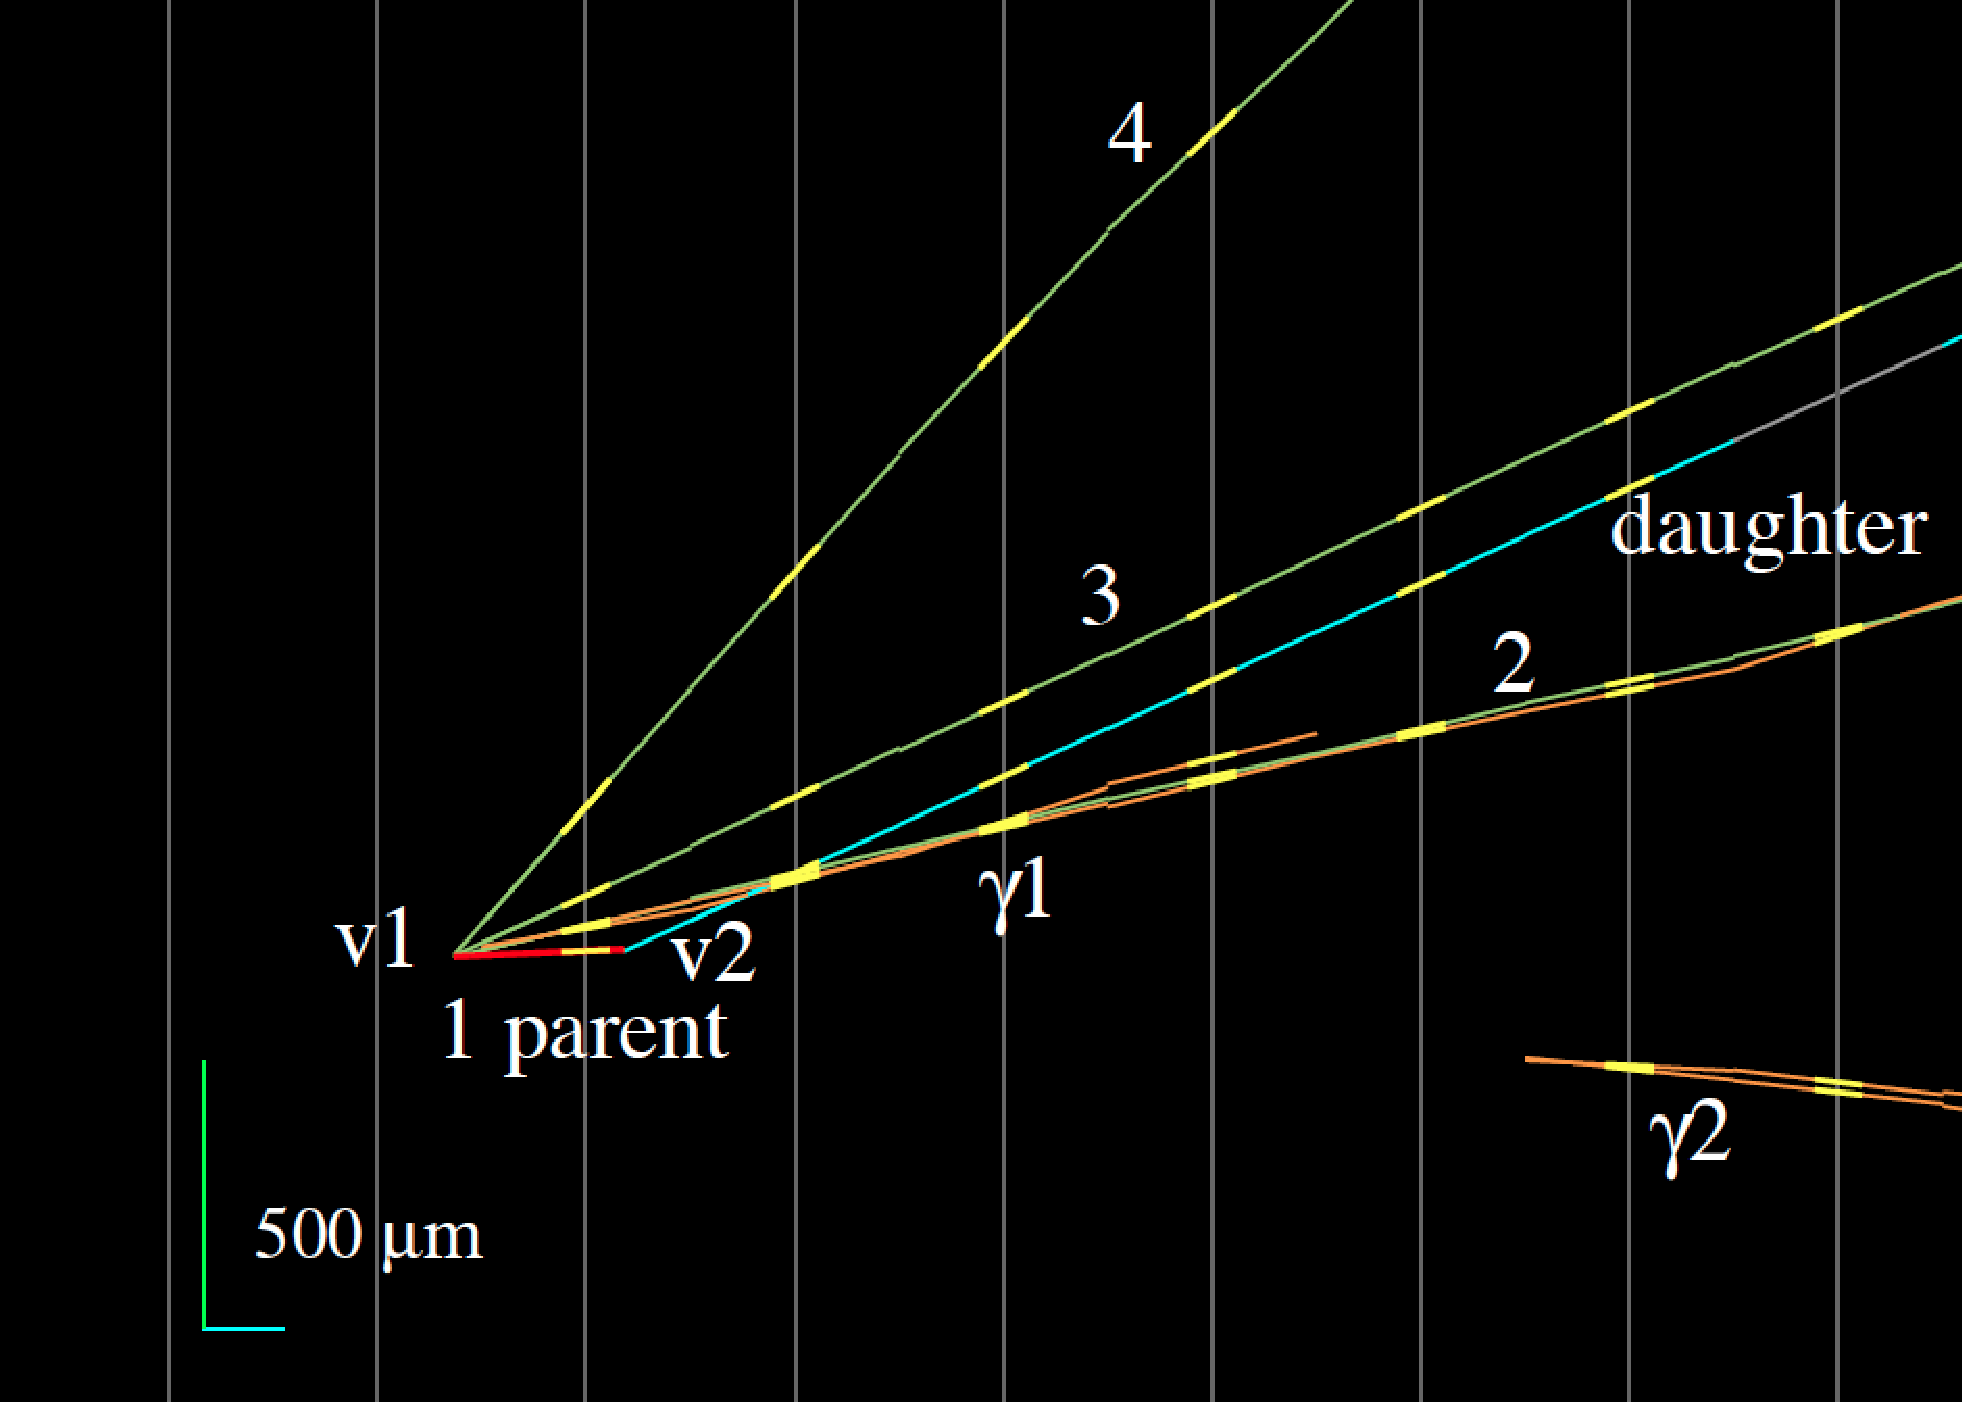
\includegraphics[width=0.5\linewidth]{figures/tau4.pdf}
  \caption{
Event display of the fourth $\nu_\tau$ candidate event from the OPERA 
experiment~\cite{DICRESCENZO2015186} in the
horizontal projection longitudinal to the neutrino direction.
The primary and secondary vertices are indicated as v$_1$ and
v$_2$ , respectively. The kink between the parent and daughter track, a feature of $\tau$ lepton decays, is clearly visible. The yellow stubs represent the track segments as measured in the emulsion films.  Courtesy of the OPERA collaboration.
}
 \label{fig:opera}
 \end{figure}

